\documentclass{article}

% Packages
\usepackage[utf8]{inputenc} % For modern characters
\usepackage{microtype} % For sexy kerning
\usepackage{mathtools} % For math stuff
\usepackage{amssymb} % For math symbols
\usepackage{tabularx} % For making tables
\usepackage{fancyhdr} % Use a header
\usepackage{pdfpages} % For including a graphics path

% Set the margins
\usepackage[scale=0.8, top=1in, bottom=1in]{geometry}

% Other front matter
\graphicspath{ {img/} } % Put all images in img/
\newcommand{\code}[1]{\texttt{#1}} % More readable for writing inline code.
\newcommand{\p}[1]{\paragraph{#1}} % Easier to type out for paragraph command
\newcommand{\addsection}[1]{\addcontentsline{toc}{section}{#1}} % content lines
\newcommand{\addsubsection}[1]{\addcontentsline{toc}{subsection}{#1}} % content lines
\pagestyle{fancy} % Makes Header Possible
{ %%% Header Set up
	\lhead{} % Set the left header to be blank
	\chead{} % Set the center header to be blank
	% Header for every page except the first two
	\rhead{Ben Foster | Lab 5 | May 22, 2015} % Name, assignment, date
}
\setcounter{tocdepth}{2} % Set Table of Contents Depth
\setlength{\parindent}{0pt} % Disable automatic indentation

%%%%%%%%%%%%%%%%%%%%% Begin Document %%%%%%%%%%%%%%%%%%%%%
\begin{document}

{ % Title page, table of contents, and page number setting
	\title{Probability and Statistics for Engineers Lab Five \\ TMATH 390}
	\author{Ben Foster\thanks{
		Institute of Technology, University of Washington Tacoma} \\
		Instructor: Julia Eaton}
	\date{May 22, 2015} % Include the date
	\maketitle % Make the title
	\thispagestyle{empty} % No page number at bottom
	\clearpage % Start the table of contents on the next page
	
	\pagenumbering{roman} % Use roman numerals for numbering
	\tableofcontents % Make the table of contents
	\clearpage % Start homework on next page
	\setcounter{page}{1} % Begin numbering over again
	\pagenumbering{arabic} % use arabic numerals for numbering
}

\section*{Part 1}
\addsection{First Part}

Sampling distribution of the sample mean, when population is normal.

\begin{center}
	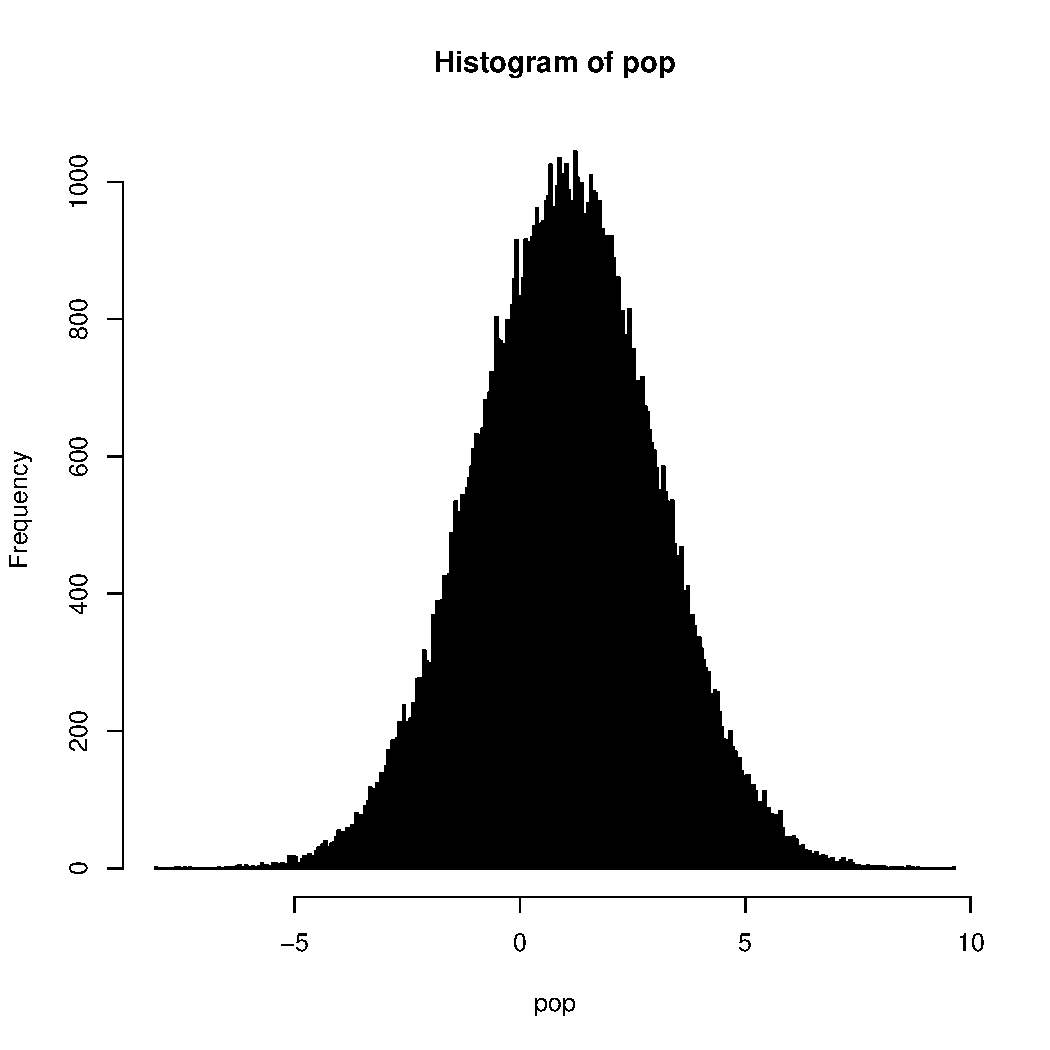
\includegraphics[width=\textwidth]{Lab5_1.pdf}
	\addsubsection{Histogram of First Population}
\end{center}

The mean of the sample mean I got was 0.9992485. This is very close to the population mean (0.9955118) but is slightly higher. \\

The standard deviation of the sample mean I got was 0.638113 while $\frac{\text{population standard deviation}}{\sqrt{n}} = 0.6346838$ which is very close together.


\begin{center}
	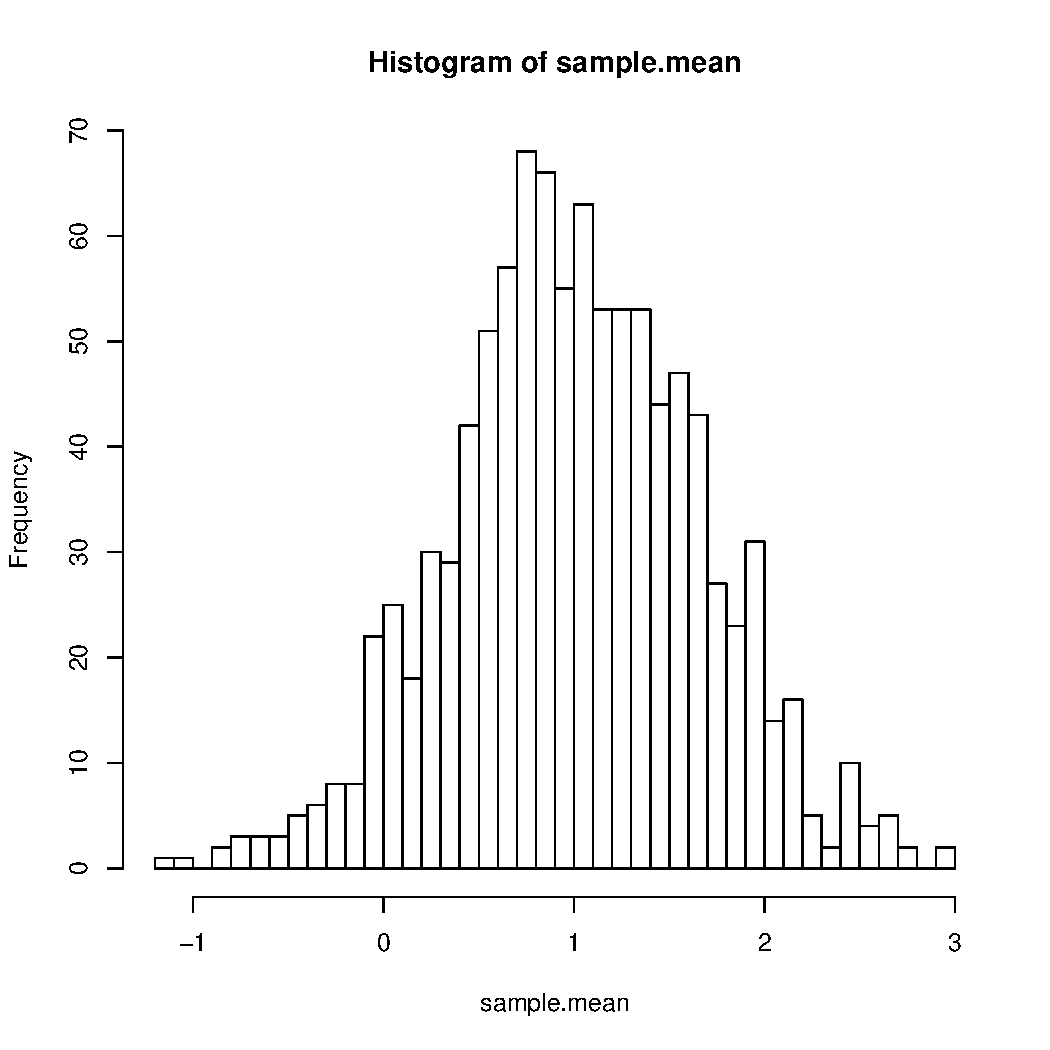
\includegraphics[width=\textwidth]{Lab5_2.pdf}
	\addsubsection{Histogram of First Sample Mean}
\end{center}
\begin{center}
	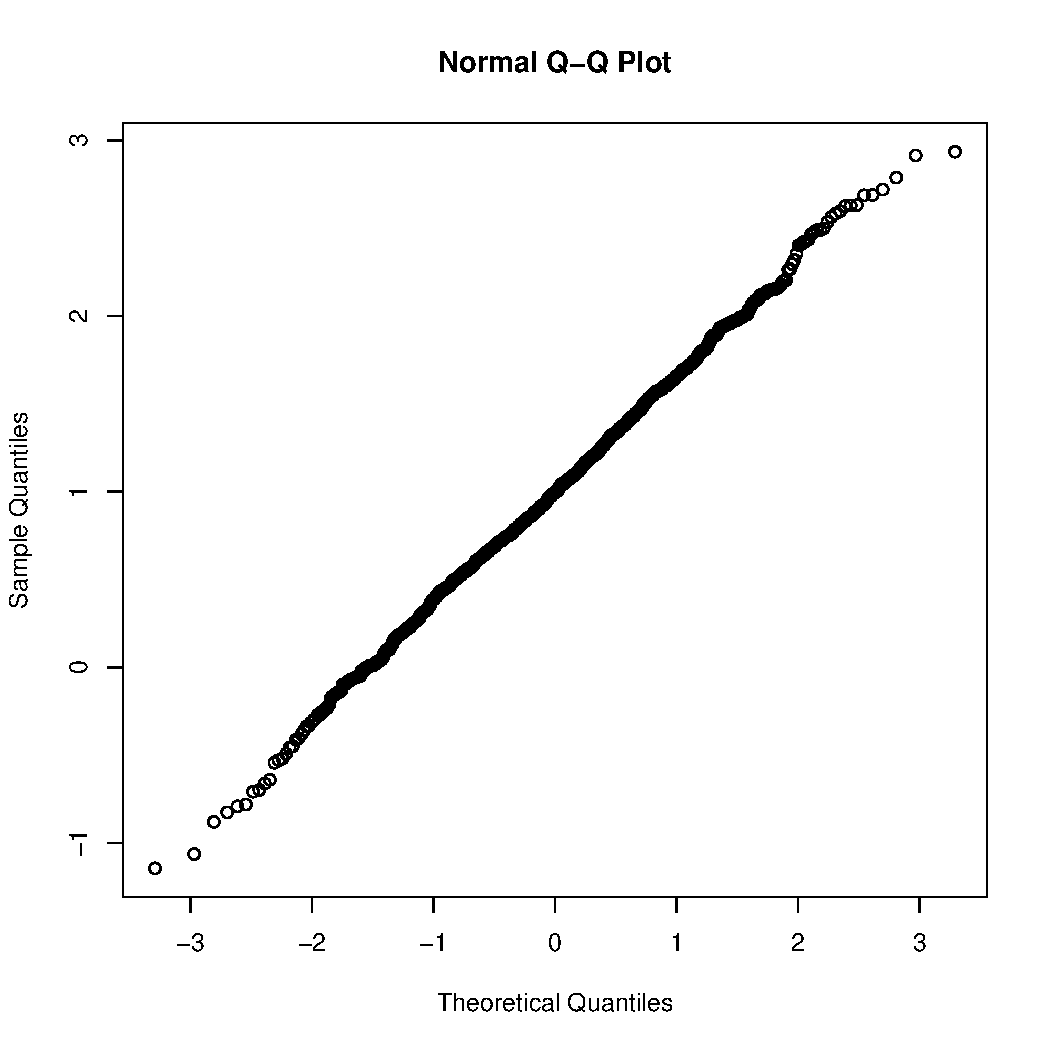
\includegraphics[width=\textwidth]{Lab5_3.pdf}
	\addsubsection{First Normal Q-Q Plot}
\end{center}

\clearpage
\section*{Part 2}
\addsection{Second Part}

Sampling distribution of the sample mean, when population is NOT normal.

\begin{center}
	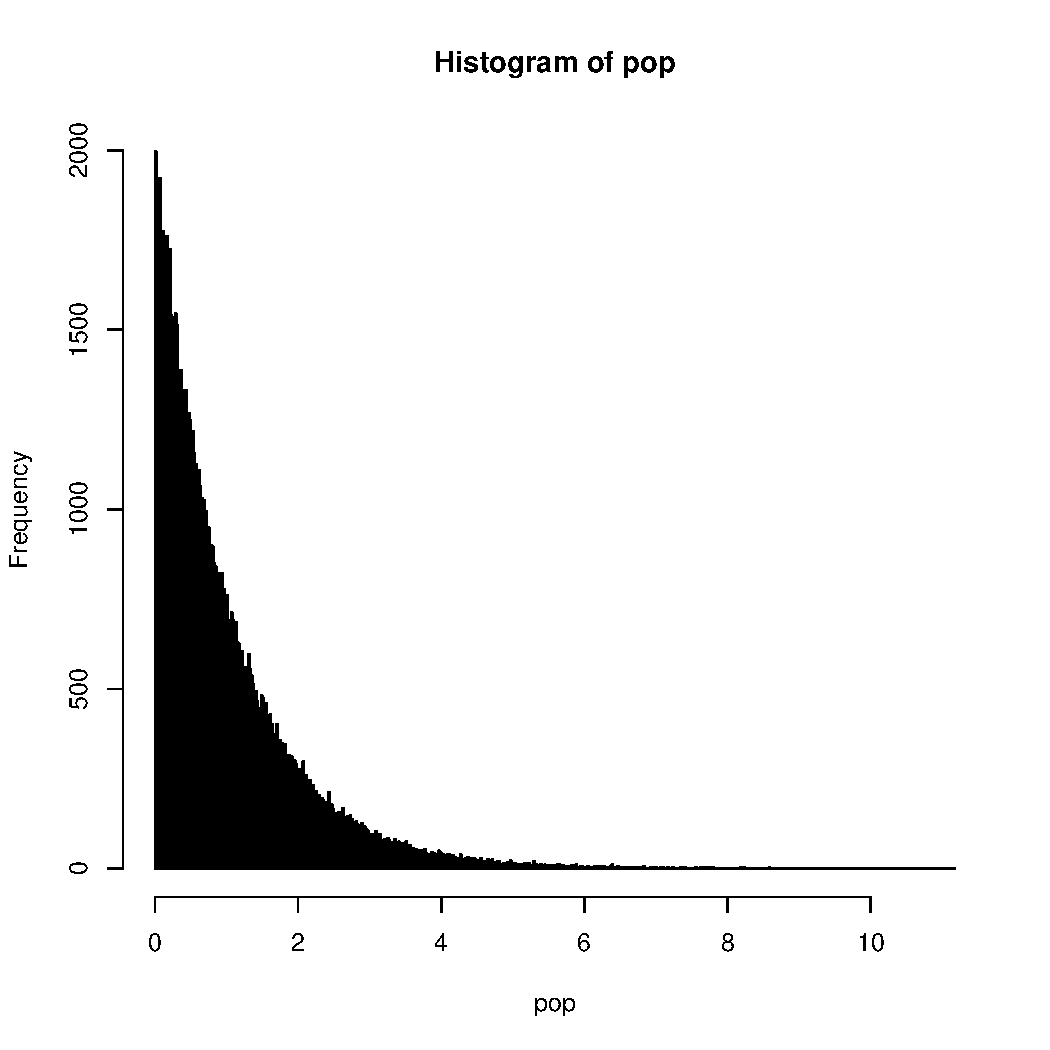
\includegraphics[width=\textwidth]{Lab5_4.pdf}
	\addsubsection{Histogram of Second Population}
\end{center}

The calculated mean of sample means I got was 1.003286 while the population mean was 0.9955118. Very close together but not exact. \\

Once again, the population standard deviation and the standard deviation of the sample mean were completely different, but when comparing the standard deviation of the sample mean with $\frac{\text{population standard deviation}}{\sqrt{n}}$ (0.3168481 and 0.3165026 respectively) we get values much closer to each other.

\begin{center}
	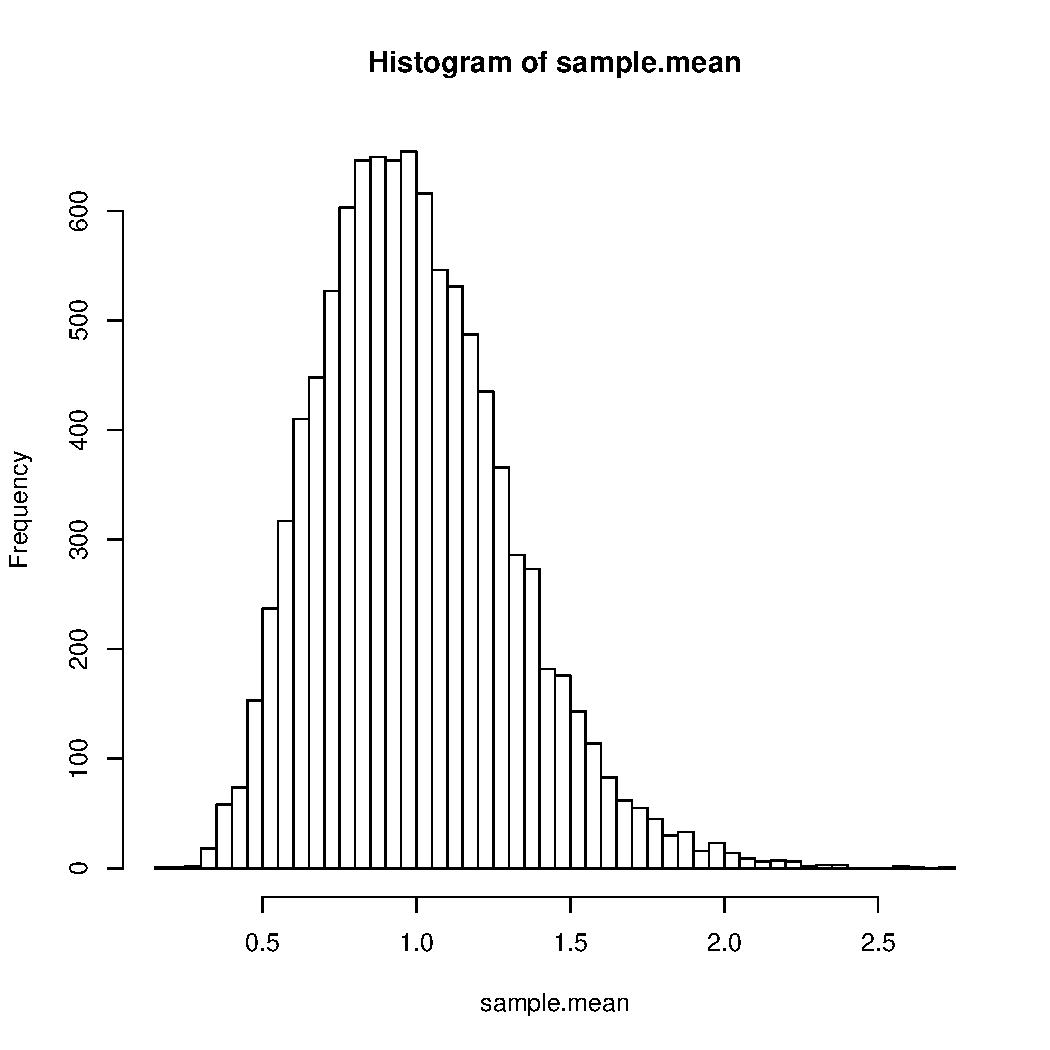
\includegraphics[width=\textwidth]{Lab5_5.pdf}
	\addsubsection{Histogram of Second Sample Mean}
\end{center}
\begin{center}
	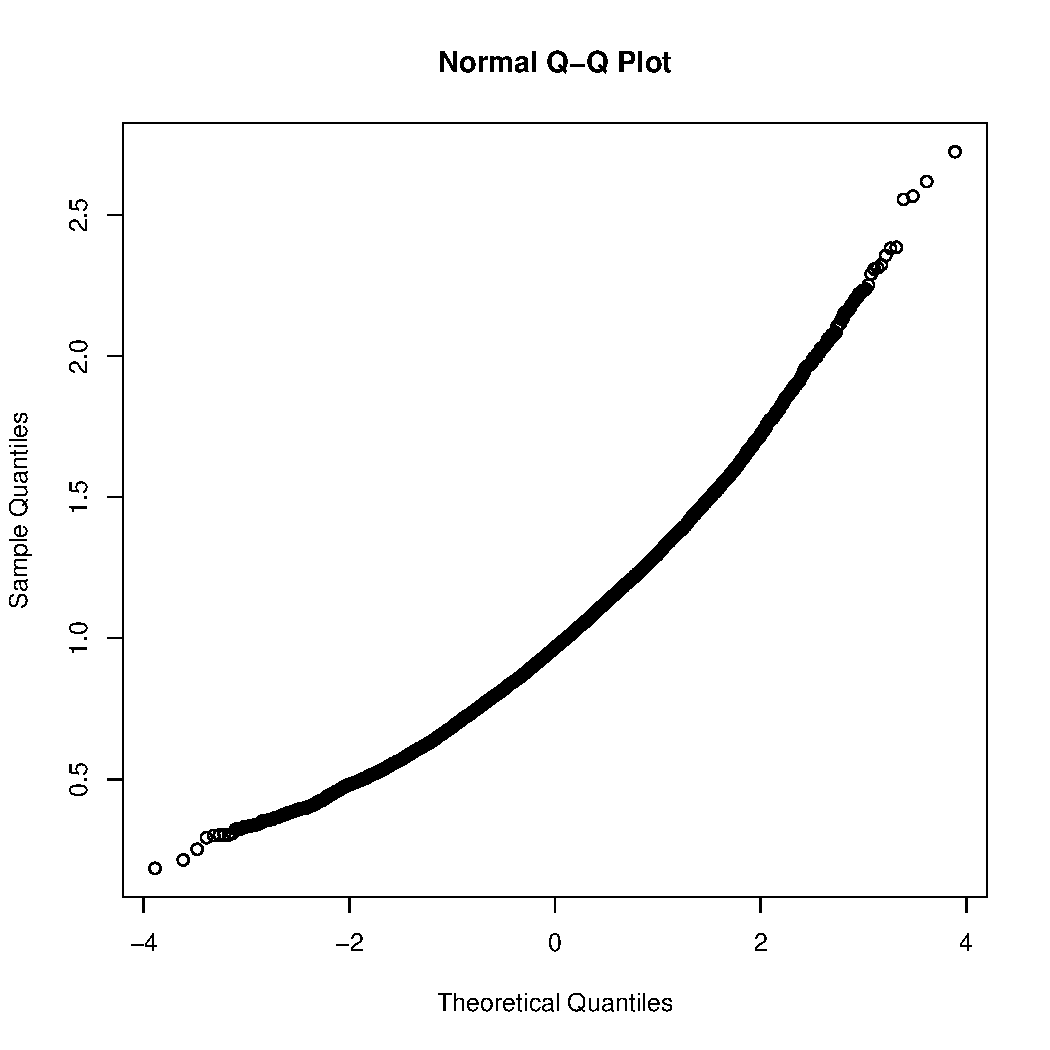
\includegraphics[width=\textwidth]{Lab5_6.pdf}
	\addsubsection{Second Normal Q-Q Plot}
\end{center}

\clearpage
\p{Repeated graphs for sample.size = 100}

\begin{center}
	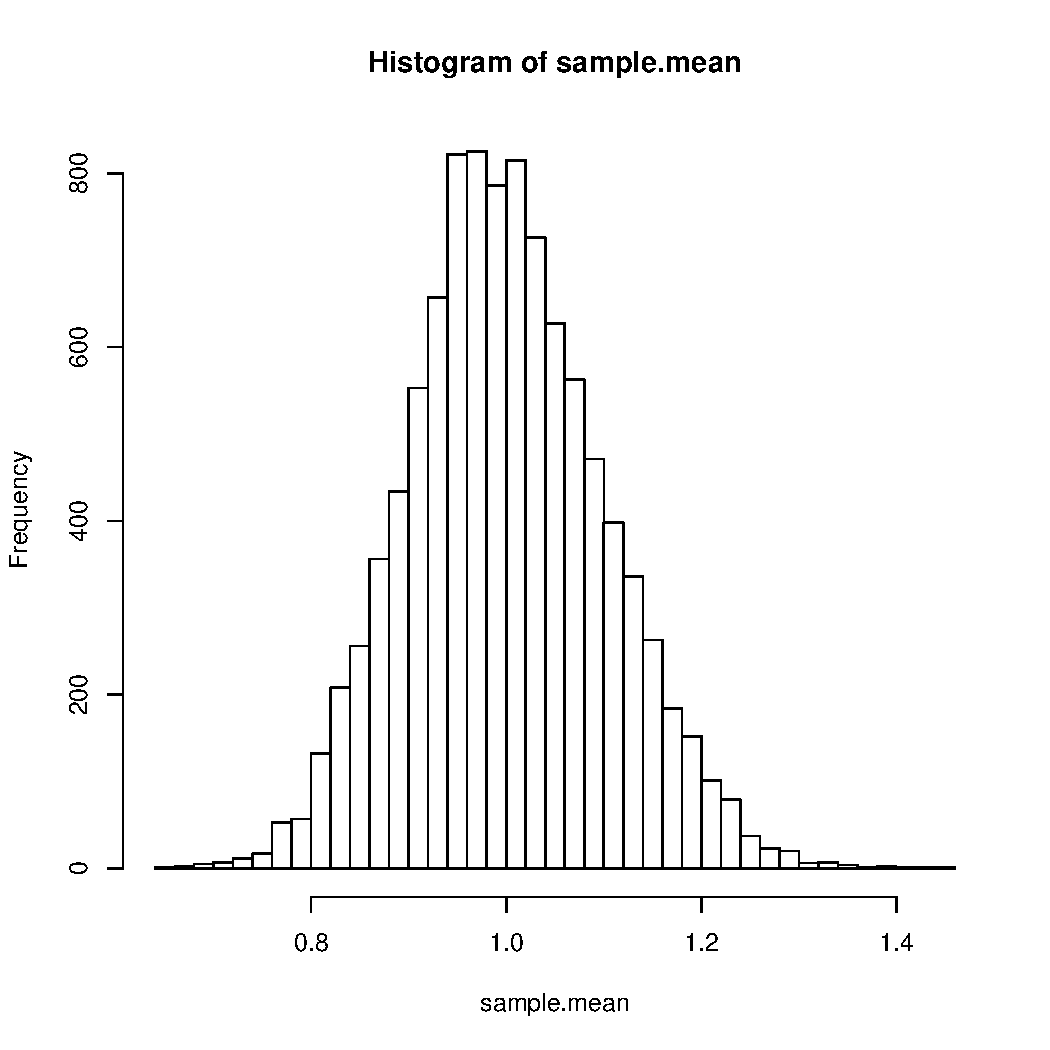
\includegraphics[width=\textwidth]{Lab5_7.pdf}
	\addsubsection{Repeated Histogram With Different Sample Size}
\end{center}
\begin{center}
	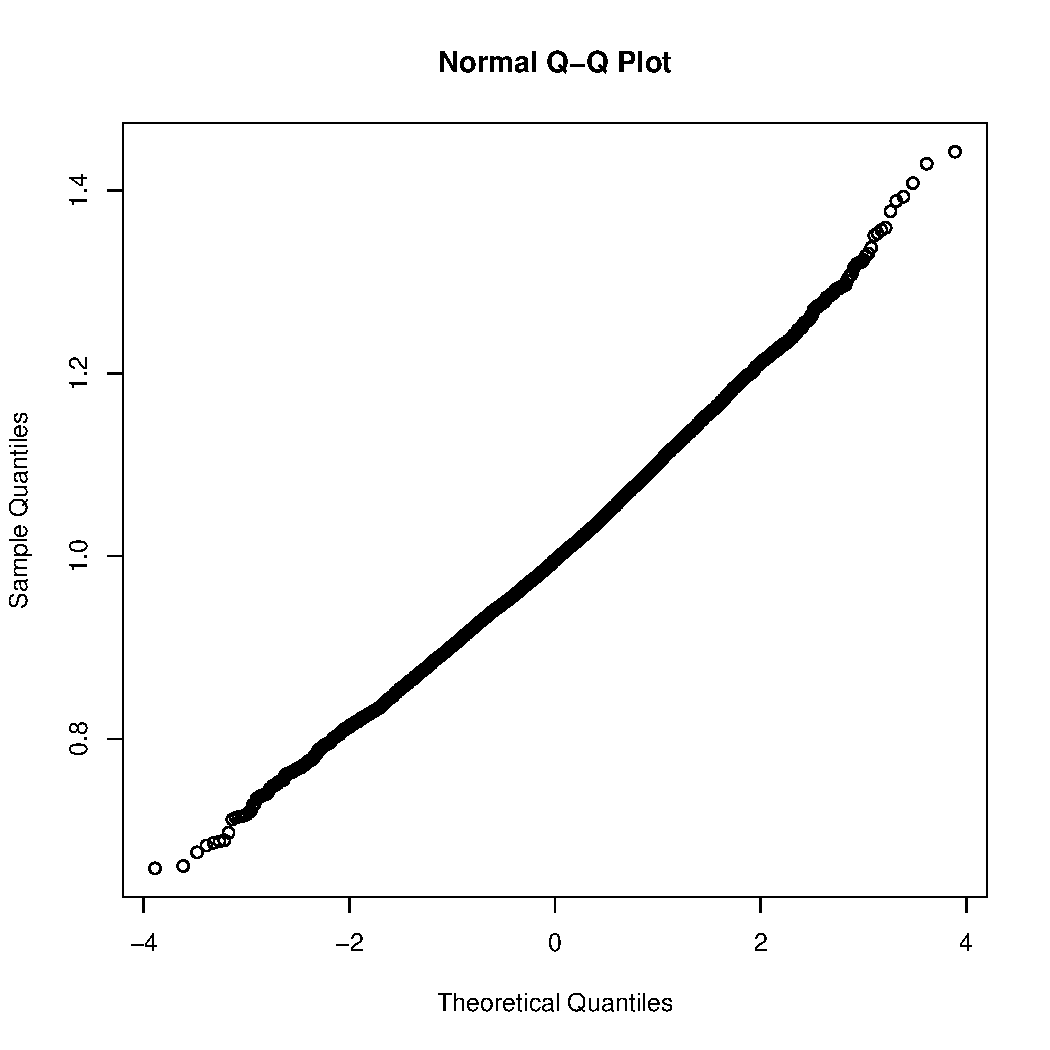
\includegraphics[width=\textwidth]{Lab5_8.pdf}
	\addsubsection{Repeated Normal Plot With Different Sample Size}
\end{center}

\clearpage
\section*{Part 3}
\addsection{Third Part}

What are the mean and standard deviation of the sampling distribution of the sample median? \\
What is the sampling distribution of the sample median itself? \\

In this case, the mean of sample medians was 0.7446777 compared to the population median of 0.6978674, these numbers are relatively very different.

\begin{center}
	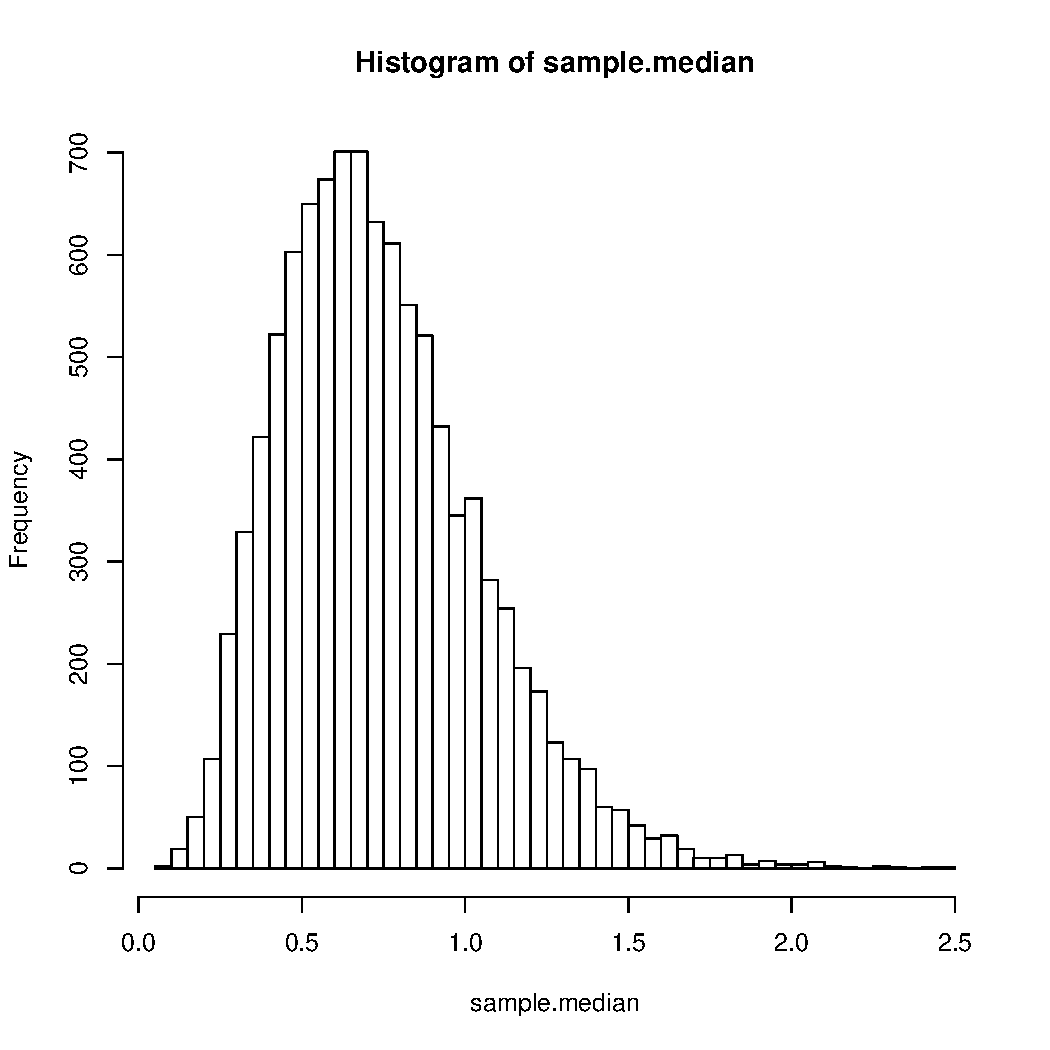
\includegraphics[width=\textwidth]{Lab5_9.pdf}
	\addsubsection{Histogram of Third Sample Median}
\end{center}
\begin{center}
	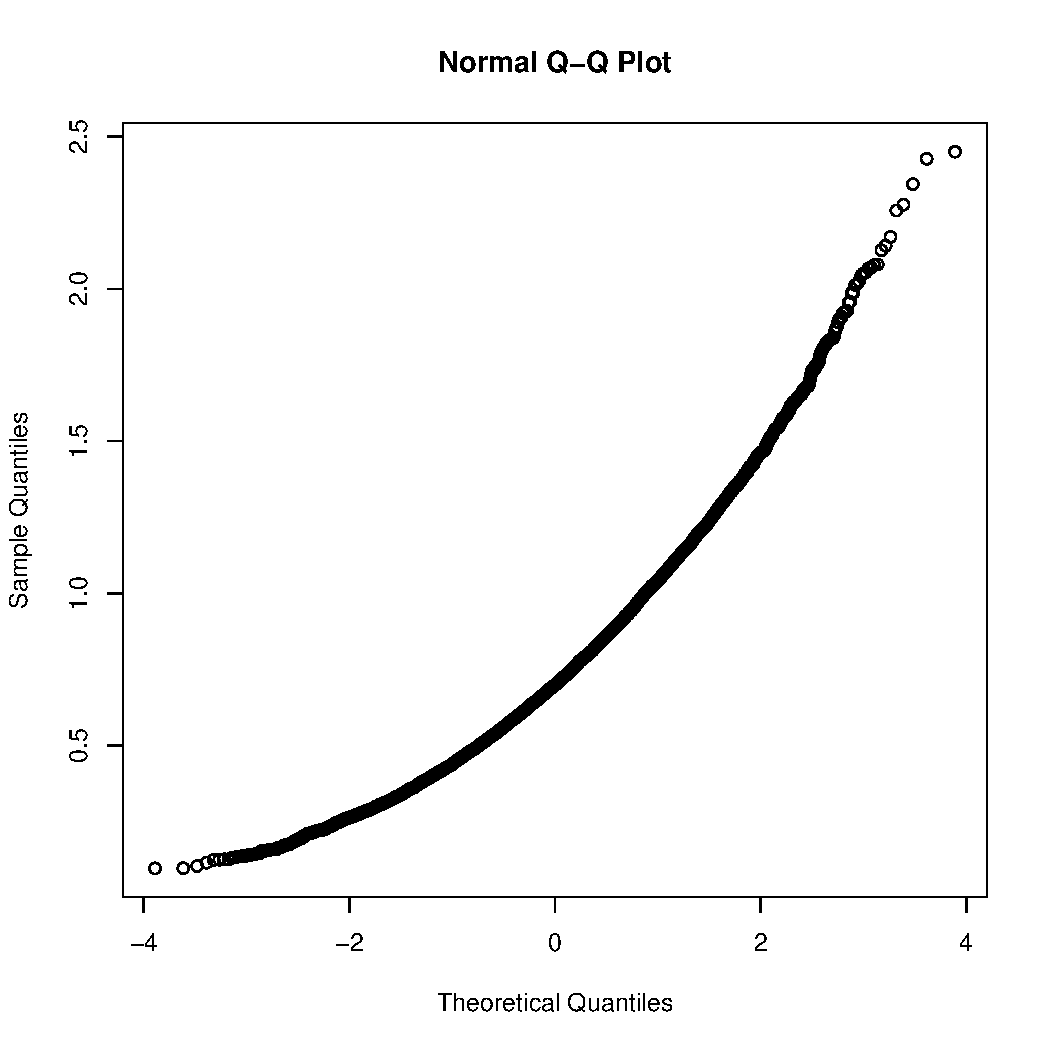
\includegraphics[width=\textwidth]{Lab5_10.pdf}
	\addsubsection{Third Normal Q-Q Plot}
\end{center}

\clearpage
\p{Repeated graphs for sample.size = 100}

\begin{center}
	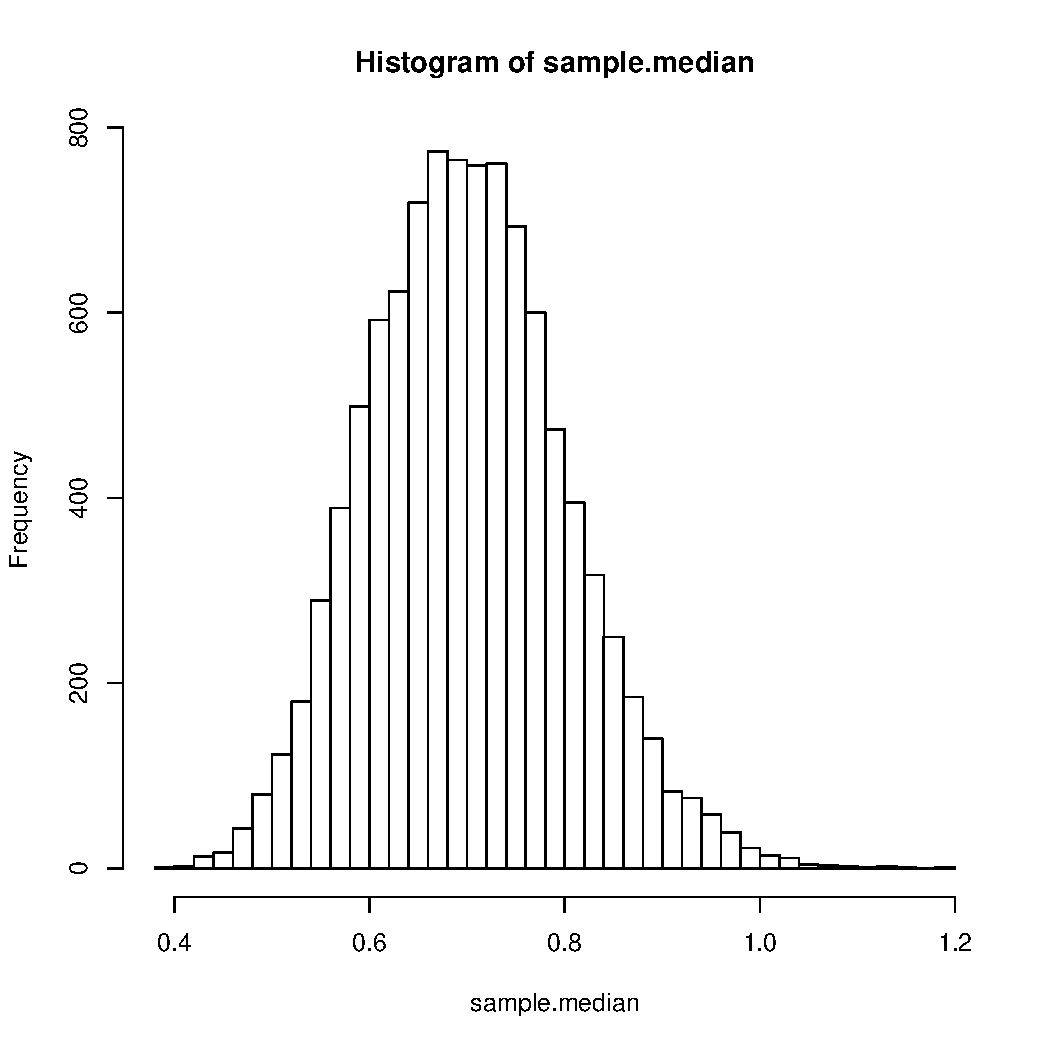
\includegraphics[width=\textwidth]{Lab5_11.pdf}
	\addsubsection{Repeated Histogram With Different Sample Size}
\end{center}
\begin{center}
	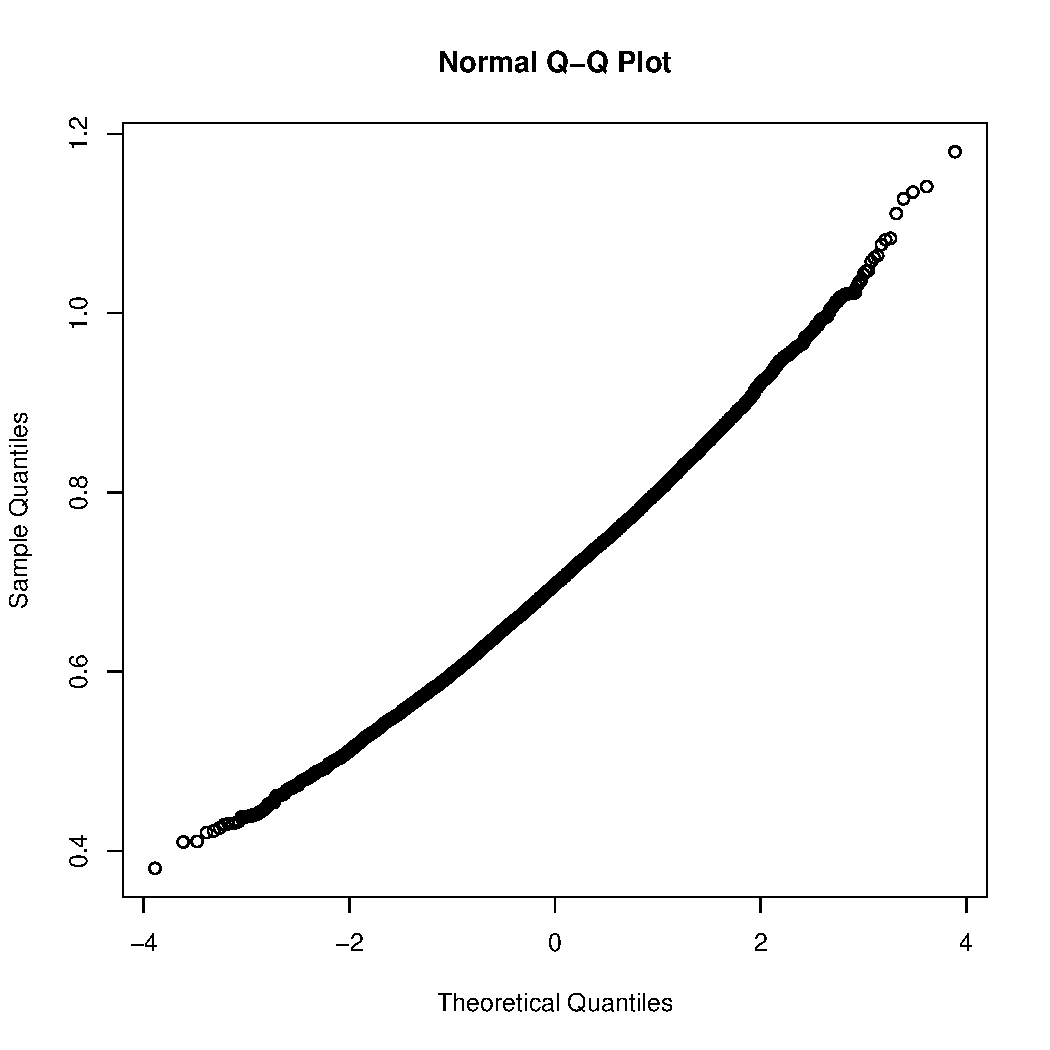
\includegraphics[width=\textwidth]{Lab5_12.pdf}
	\addsubsection{Repeated Normal Plot With Different Sample Size}
\end{center}

\section*{Part 4}
\addsection{Fourth Part}

Confidence interval for population mean. \\
By using the code given, the determined confidence interval was (0.9548423, 1.2874648) with a mean of x being equal to 1.121154.

\clearpage
\section*{Part 5}
\addsection{Fifth Part}

Coverage of a Confidence Interval.

\begin{center}
	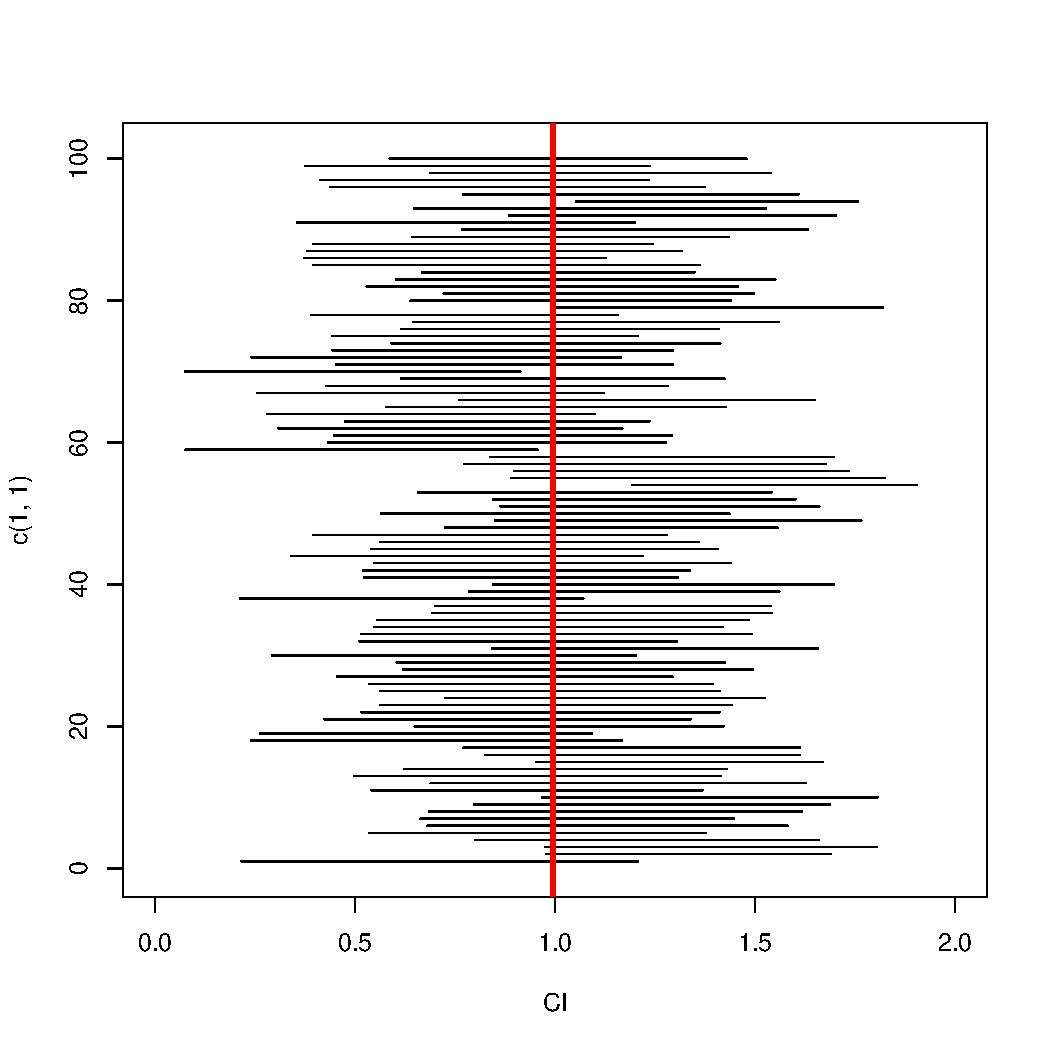
\includegraphics[width=\textwidth]{Lab5_13.pdf}
	\addsubsection{Graph of the Coverage of a Confidence Interval}
\end{center}

	
\end{document}